\subsection{Heurística Simmulated Annealing}

\subsubsection{El algoritmo}
Dada una función de distancia total, podemos calcular la utilidad de cada función, sabiendo que a menor distancia total, mejor es la solución. El dominio de esta función equivale a todas las solución posibles de de un problema de VRP, por lo que explorar la totalidad del dominio en busca del mínimo resulta inviable.

Sin embargo, partiendo de una solución aceptable encontrada por otra heurística, podemos tratar de explorar soluciones cercanas, en busca de hallar una mejor solución. Repitiendo este proceso buscamos minimizar la solución en función de la distancia total, llegando al mínimo global. Ver \textit{figura \ref{fig:convergencia}}

Para esto existe una gran cantidad de algoritmos, entre ellos:

\begin{itemize}\itemsep0em
\item Hill Climbing
\item Gradient Descent
\item Grasp
\item Tabu Search
\end{itemize}

Sin embargo, al hablar de VRP, nuestro dominio resulta ser más complejo, dando lugar a mínimos locales, en donde nuestro algoritmo puede quedar atrapado. Ver \textit{figura \ref{fig:minimo-local}}


\begin{figure}[H]
	\centering
	\begin{minipage}[t]{.45\textwidth}
		\centering
		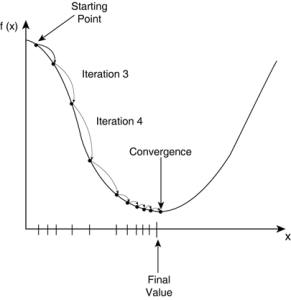
\includegraphics[scale=0.55]{annealing/fig1}
		\caption{Convergencia hacia el mínimo}
		\label{fig:convergencia}
	\end{minipage}\qquad
	\begin{minipage}[t]{.45\textwidth}
		\centering
		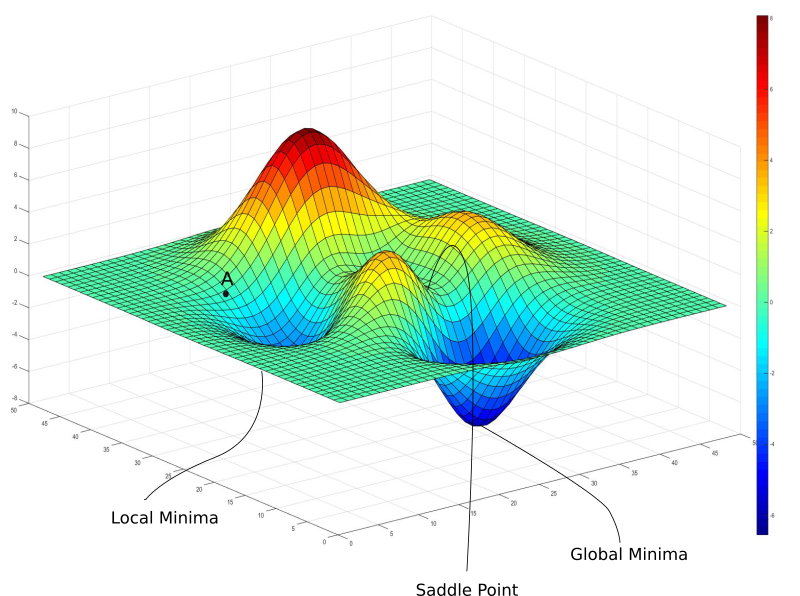
\includegraphics[scale=0.3]{annealing/fig2}
		\caption{Convergencia hacia el mínimo}
		\label{fig:minimo-local}
	\end{minipage}
\end{figure}	

Aquí es donde entra en escena Annealing, una metaheurística que trata de escaparse de los mínimos locales aceptando soluciones peores que la actual esperando desde esa peor solución llegar a una nueva que valga la pena.

El criterio que se utiliza para aceptar soluciones malas está basado en la práctica metalúrgica del recocido o \textbf{Anealing} en inglés.


Al moldear metales, se los calienta a temperaturas muy altas para poder ser moldeado, luego es enfriado para que vuelva a tomar las propiedades de rigidez y dureza. Algo parecido se busca obtener de la exploración de soluciones con está técnica.
Utilizando una temperatura artificial basada en propiedades de la solución vamos a definir cuán propensos somos a aceptar una solución mala, siguiendo el criterio de aceptar peores soluciones a mayor temperatura hasta gradualmente solo aceptar buenas soluciones una vez que nuestra temperatura se “enfríe”.


Existen múltiples versiones para la metaheurística de Annealing. a continuación presentamos el pseudocódigo para la versión reducida y la versión propuesta por Ibrahim Osman, la cual incluye resets de temperatura al llegar a caminos sin salida.

En general, las componentes comunes a las diferentes implementaciones de annealing son las siguientes:

\begin{itemize}
\item Función de energía: Define la calidad de la solución, cuanto menos tenga mejor. Se busca minimizar la energía.
\item Probabilidad de aceptación: Define la probabilidad de aceptar una solución propuesta, varía según la temperatura
\item Modificación de temperatura: Se aumenta o reduce la temperatura según la iteración y solución actual
\item Vecinos: La generación de soluciones vecinas depende del problema, se busca hacer modificaciones pequeñas.
\item Azar: Si bien utilizamos una función que nos devuelve la probabilidad de aceptar una solución, debemos comparar esa probabilidad contra un valor uniformemente aleatorio, esto significa que ejecutar el algoritmo con los mismos parámetros puede producir resultados diferentes.
\end{itemize}

\subsubsection{Pseudocodigo}

\begin{algorithm}[H]
\caption{Simple Simmulated Annealing}
\begin{algorithmic}[1]
\Function{Anneal}{Solucion $S_0$, Entero $T_{max}$, Entero $T_{min}$} \Comment $\Theta()$
\State $S \gets S_0$ \Comment $\Theta(1)$
\State $S_b \gets S_0$ \Comment $\Theta(1)$
\State $T \gets T_{max}$ \Comment $\Theta(1)$
\State
\While{$T > T_{min}$} \Comment $\Theta()$
	\State $S' \gets \textit{Vecino(S)}$ \Comment $\Theta()$
	\If{$\textit{ProbabilidadDeAceptar(S, S', T)} \geq \textit{Random(0, 1)} $} \Comment $\Theta()$
		\State $S \gets S'$ \Comment $\Theta(1)$
	\EndIf	
	\State
	\If{$\textit{Energia(S)} < \textit{Energia}(S_b)$} \Comment $\Theta()$
		\State $S_b \gets S$ \Comment $\Theta(1)$
	\EndIf	
	\State \textit{Enfriar(T)} \Comment $\Theta()$
\EndWhile
\State
\State \Return $S_b$ \Comment $\Theta(1)$
\EndFunction
\end{algorithmic}
\end{algorithm}

Como podemos ver, en esta versión de Annealing, establecemos un rango de temperaturas dentro del cual operar, explorando soluciones lindantes a la actual y aceptandolas de acuerdo a una probabilidad en función de la temperatura actual y la calidad de dicha solución.


Esto nos permite fácilmente tratar de minimizar nuestra solución inicial $S_0$, pero corremos el riesgo de quedar atrapados en un mínimo local según la probabilidad de aceptar una solución al azar.

Para combatir esto, decidimos seguir casi al pie de la letra la versión de Annealing descrita por \textit{Osman} en su paper, la cual al llegar a un camino sin salida, retrocede hasta la mejor solución encontrada, eleva la temperatura y prueba nuevamente de minimizar la solución, esperando esta vez seguir un camino diferente.


\begin{figure}[H]
	\centering
	\begin{minipage}[t]{.45\textwidth}
		\centering
		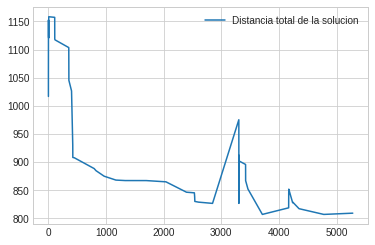
\includegraphics[scale=0.55]{annealing/distancia-total}
	\end{minipage}\qquad
	\begin{minipage}[t]{.45\textwidth}
		\centering
		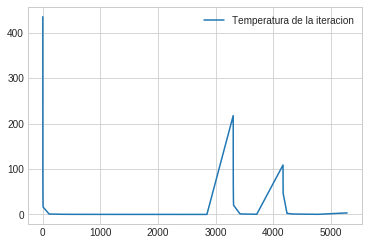
\includegraphics[scale=0.55]{annealing/temperatura}
	\end{minipage}
	
	Podemos ver como al elevarse la temperatura, se logra escapar de caminos sin salida, los cuales hubiesen sido devueltos como solución final por la implementación sencilla.
\end{figure}	


\begin{algorithm}[H]
\caption{Simmulated Annealing with Temperature Cycles}
\begin{algorithmic}[1]
\Function{Anneal}{Solucion $S_0$, Entero $R$} \Comment $\Theta()$
\State $S \gets S_0$ \Comment $\Theta(1)$
\State $S_b \gets S_0$ \Comment $\Theta(1)$
\State $T_s, T_f  \gets \textit{CalcularRangoDeTemperatura(S)}$ \Comment $\Theta(1)$
\State $T_k \gets T_{s}$ \Comment $\Theta(1)$
\State $resets \gets 0$ \Comment $\Theta(1)$
\State $k \gets 0$ \Comment $\Theta(1)$
\State
\While{$resets < R$} \Comment $\Theta()$
	\State $k \gets k + 1$ \Comment $\Theta(1)$
	\State
	\If{$\textit{HayVecinos(S)}$} \Comment $\Theta()$
		\State $\Delta_{energia} \gets \textit{ProximoVecino(S)}$ \Comment $\Theta()$
		\If{$\textit{ProbabilidadDeAceptar}(\Delta_{energia} , T_k) \geq \textit{Random(0, 1)} $} \Comment $\Theta()$
			\State $S \gets \textit{AceptarVecino(S)}$ \Comment $\Theta()$
		\EndIf
		\If{$\textit{Energia(S)} < \textit{Energia}(S_b)$} \Comment $\Theta()$
			\State $S_b \gets S$ \Comment $\Theta(1)$
			\State $resets \gets 0$ \Comment $\Theta(1)$
		\EndIf	
		\State \textit{Enfriar($T_k$, $t_s$, $t_f$, $k$)} \Comment $\Theta()$		
		\State
	\Else
		\State \textit{Calentar($T_k$, $t_s$, $t_f$, $k$)} \Comment $\Theta()$			
		\State $resets \gets resets + 1$ \Comment $\Theta(1)$
		\State \textit{GenerarNuevosVecinos(S)} \Comment $\Theta(1)$
	\EndIf

\EndWhile
\State
\State \Return $S_b$ \Comment $\Theta(1)$
\EndFunction
\end{algorithmic}
\end{algorithm}

Para poder entender el algoritmo, debemos conocer las siguientes funciones:

\begin{description}
\item[Energia] devuelve el la distancia total recorrida por los camiones en una solución, buscamos minimizarla

\item[CalcularRangoDeTemperatura] explora un vecindario completo de la solución y devuelve el mayor y menor cambio de energía encontrado

\item[HayVecinos] indica si quedan soluciones vecinas por explorar

\item[ProximoVecino] devuelve el la diferencia de energía entre la solución actual y el próximo vecino

\item[AceptarVecino] modifica la solución actual para reflejar el último vecino consultado

\item[ProbabilidadDeAceptar] dependiendo de la temperatura actual y la diferencia en energía propuesta, devuelve cierta probabilidad de que la solución sea aceptada (notar que el hecho de que sea aceptada o no, depende de que esta probabilidad sea mayor al número aleatorio contra el cual se compara) Esta sigue la fórmula:
$$ P = \mathlarger{\mathlarger{e^\frac{-\Delta_{energia}}{T_k}}} $$

\item[Enfriar] en base al rango de temperaturas de la solución inicial, la temperatura actual, iteración y otros parámetros, decrementa el valor de la temperatura actual, forzando a que la función “probabilidadDeAceptar” devuelva cada vez valores más bajos para una solución con un cambio de energía positivo (es decir, una solución peor a la actual)
esta sigue la formula: 
$$ T = \frac{T_k}{1+ \beta_k T_k},  \beta_k = \frac{T_s - T_f}{(\alpha + \gamma \sqrt{k} )T_s T_k} $$

\item[Calentar] eleva la temperatura actual a la temperatura que sea mayor entre la temperatura para la cual fue encontrada la mejor solución y la mitad de la temperatura del último reset

\item[NuevosVecinos] vuelve a recrear el vecindario de soluciones, para que pueda volver a ser explorado
\end{description}

Por ultimo, es necesario dar una explicación sobre la exploración del vecindario. Siguiendo lo propuesto por \textit{Ibrahim Osman}, utilizamos el metodo de exploracion Lambda-interchange para generar vecinos. Este método propone recorrer de manera aleatoria todas las combinaciones posibles entre camiones, y para cada una de ellas generar todos los intercambios posibles entre puntos según las siguientes operaciones.

Dadas dos rutas Rp y Rq, definimos:

\begin{description}
\item[Left shift:] Tomamos un punto de la ruta Rq y lo insertamos en la ruta Rq. está operación puede eliminar rutas

\item[Right shift:] Tomamos un punto de la ruta Rq y lo insertamos en la ruta Rp. está operación puede eliminar rutas

\item[Exchange:] Intercambiamos punto de la ruta Rq con uno de la ruta Rq
\end{description}

Esto nos permite generar un vecindario iterable de soluciones, el cual utilizamos para minimizar la energía.


\subsubsection{Peores Casos}

La metaheurística de annealing se ve afectada por 3 factores que determinan qué tan probable es encontrar una solución óptima. Estos son la solución inicial, la forma del plano de la distancia total de las soluciones y el azar.

Annealing parte de una solución inicial ya calculada y de esta deriva la temperatura inicial y final por lo que cuando solución inicial es similar en energía a la solución óptima, puede resultar difícil hallar el camino entre las dos, dado que la temperatura no va a ser suficiente para escapar de los puntos silla.

\begin{figure}[H]
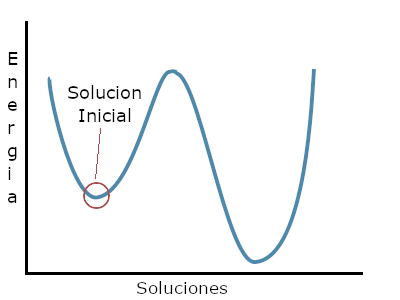
\includegraphics[scale=2]{annealing/mala-sol-inicial}
\centering
\end{figure}

Otro caso se basa en el mecanismo de exploración de vecindario, específicamente en las operaciones de intercambio. Cada camión tiene una capacidad máxima, por lo que no todas las operaciones se pueden aplicar para un conjunto de rutas y puntos.
Por ejemplo, si suponemos un camión sin capacidad disponible, entonces no va a ser posible realizar operaciones de shift que sumen puntos a su recorrido.
Un escenario complejo de este caso se da cuando no se puede realizar ninguna operación entre ningun camion, dado que cualquier punto intercambiado entre dos camiones excedería la capacidad de uno de los dos.
Si bien este escenario parece exagerado, es un escenario común (Probabilidad 1\%) para ciertos datasets particulares, o simplemente cuando el presupuesto de iteraciones para annealing es elevado.

\begin{figure}[H]
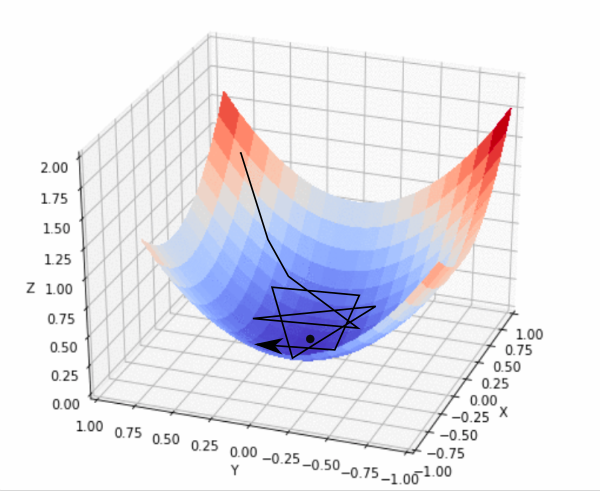
\includegraphics[scale=0.4]{annealing/rebote-convergencia}
\centering
\caption{Debido a baja temperatura y mala suerte, el algoritmo puede tardar en converger}

\end{figure}


